\documentclass[a4paper, english, 12pt]{article}
\usepackage[utf8]{inputenc}
\usepackage[norsk]{babel}
\usepackage{mathtools}
\usepackage{hyperref}
\usepackage{listings}
\usepackage{graphicx}

\begin{document}
\input{title.tex}
\section{Introduction}
This document contains the exercise description of the group exercise in TTM4100. It contains the class diagram of a simple chat server, the sequence diagrams as a short design description.

\section{Class diagram}
In our class diagram, as seen in figure \ref{class}, we have descriped several relations as listed in the following sections.

\begin{figure}[h!] 
    \begin{center}  
    	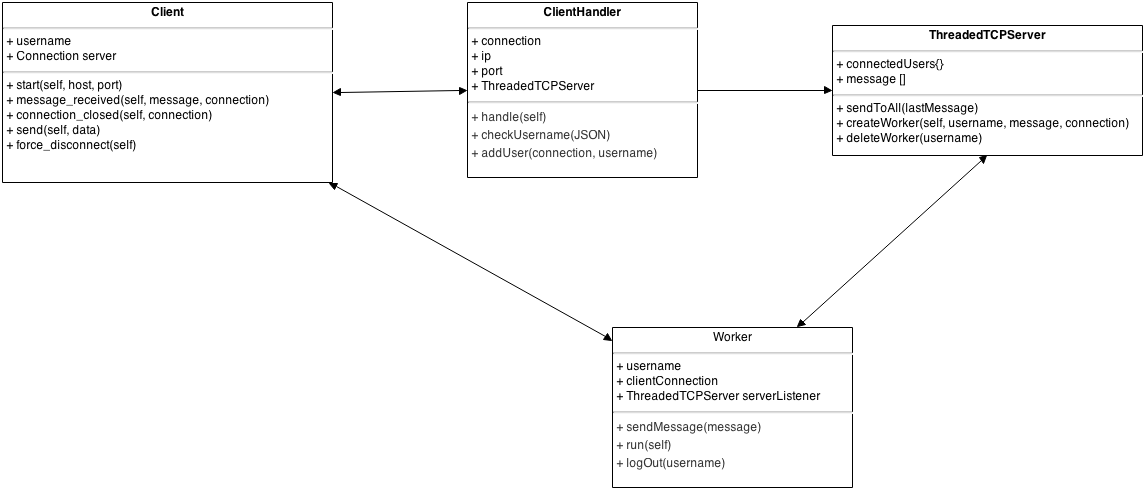
\includegraphics[width=8cm]{ktnClassDiagram.png}
		\caption{class diagram}
	\label{class}
	\end{center}
\end{figure}

\subsection{Client-CLientHandler relation}
Client sends login request to CLientHandler with desired username in a JSON format. CLientHandler performs a check on username in ThreadedTCPServer.connectedUsers\{ \} dictionary. If denied the CLientHandler will send an error message back to the Client in a JSON format. 

\subsection{Client-Worker relation}
Client sends a message to Worker in a JSON format. Client can send a logout message in a JSON format. Worker can send messages to the client in a JSON format. 

\subsection{CLientHandler-ThreadedTCPServer relation}
CLientHandler can check if a username exists in the connectedUsers dictionary in ThreadedTCPServer. CLientHandler can add a new user to connectedUsers dictionary with a connection and username.

\subsection{Worker-ThreadedTCPServer relation}
ThreadedTCPServer can create a new worker, and delete existing workers. ThreadedTCPServer can broadcast messages to all Workers. Worker informs ThreadedTCPServer of new messages. Worker informs ThreadedTCPServer when a Client has logged out.

\section{Sequence diagram}

\subsection{Login sequence diagram:}
Client connects to the server (client handler) with a JSON object.
Server checks that the username is valid and unique as shown in figur \ref{sequence}.
\begin{figure}[h!] 
    \begin{center} 
    	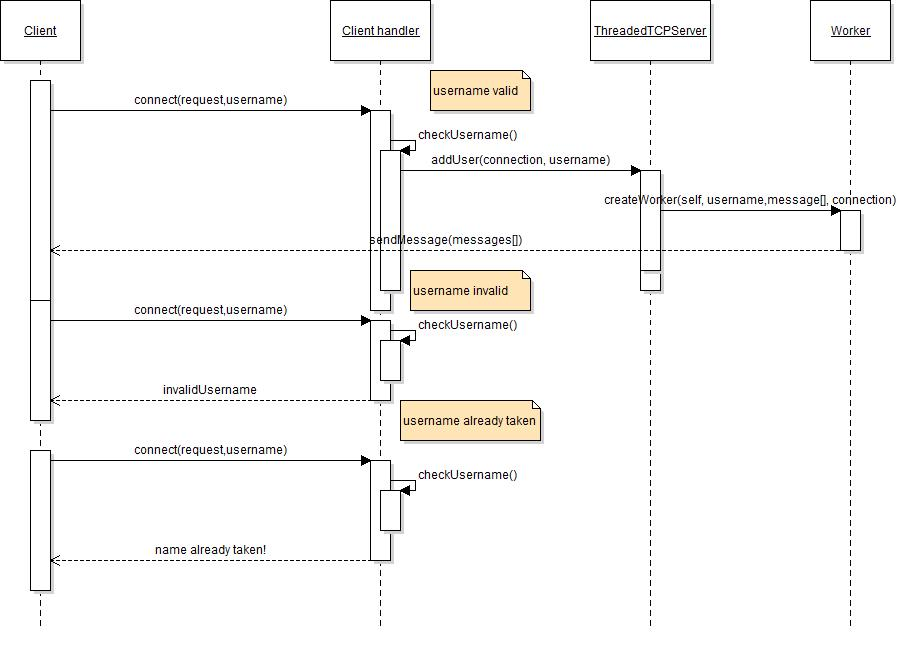
\includegraphics[width=8cm]{seqLogin.jpg}
		\caption{Sequence login}
	\label{sequence}
	\end{center}
\end{figure}

\begin{enumerate}
\item If it is valid it forwards the connection and username to ThreadedTCPServer.
Which creates a new worker and adds the username as a key in the dictionary which reffers to the worker object.
The newly created worker sends all earlier messages back to the client.
\item Invalid username, sends a error message back to the client.
\item A username already taken will also create a error message back to the client. 
\end{enumerate}



\subsection



\end{document}